Table below categorizes all the classes that appear on the sequence diagrams based on the GRASP concept they implement.
\begin{table}[H]
    \centering
    \begin{tabular}{| c | c | c | c |}
    \hline
        \textbf{Controller} & \textbf{Creator} & \textbf{Information Expert} & \textbf{Low Coupling/High Cohesion}\\
        \hline
         EventController & EventMapper & EventRepository & EventService \\
         ReviewController & EventRepository & NotificationRepository & NotificationService \\
         PostController & NotificationRepository & PostRepository & ReviewService \\
         MediaController & NotificationMapper & MediaRepository & PostService \\
           & PostRepository & PageRepository & MediaService \\
           & MediaRepository &  & DisplayService \\
           & PageRepository &  & PageService \\
           &  &  & EventMapper \\
           &  &  & NotificationMapper \\
    \hline
    \end{tabular}
    \caption{Classes with the identified GRASP concepts}
    \label{tab:my_label}
\end{table}
Low coupling and high cohesion is achieved by clearly separating out Controller, Service and Repository actions so that each class is only responsible for its specific layer of the application.  This is also a core part of the MVC pattern which is known to be loosely coupled and highly cohesive.\\
The mapper classes (EventMapper and NotificationMapper) were also identified as a creators because they are meant to be injected in service classes to create objects to be used as entities. Mapper classes support low coupling by removing a need for mapping user inputs directly to domain object needs and high cohesion by dealing only with JSON Serialization/deserialization of Event/EventDTO objects.

\subsection{Annotated Sequence diagrams}
A subset of sequence diagrams are annotated with the identified GRASP concepts and are included below. These sequence diagrams cover all the classes and the GRASP patterns they implement.

\subsubsection{Sequence Diagram: Create Event}
        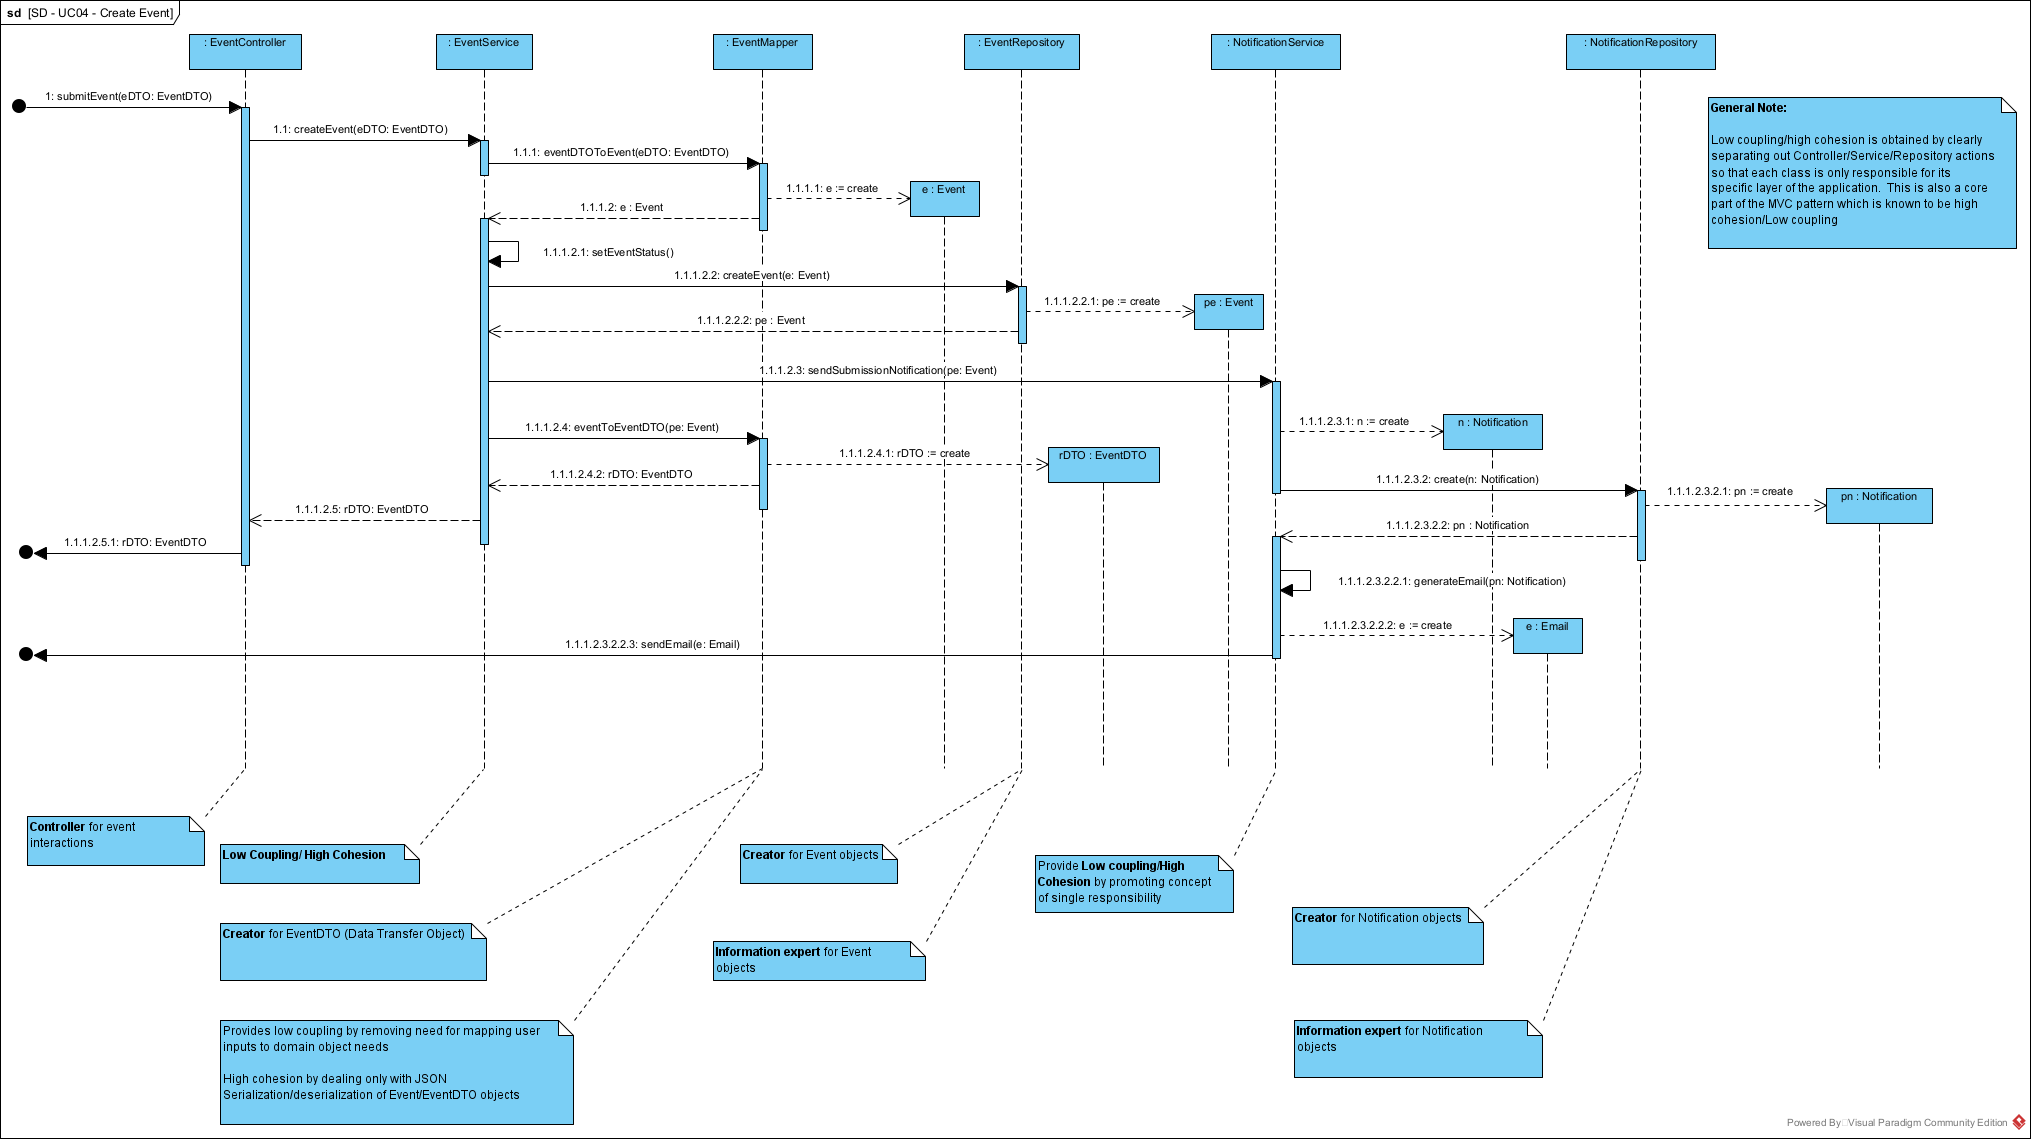
\includegraphics[scale=0.34]{images/SD-UC04-CreateEvent.png}
        \captionof{figure}{Sequence Diagram: Create Event}
        \label{fig:SD-CreateEvent}
\subsubsection{Sequence Diagram: Review for Approval}
        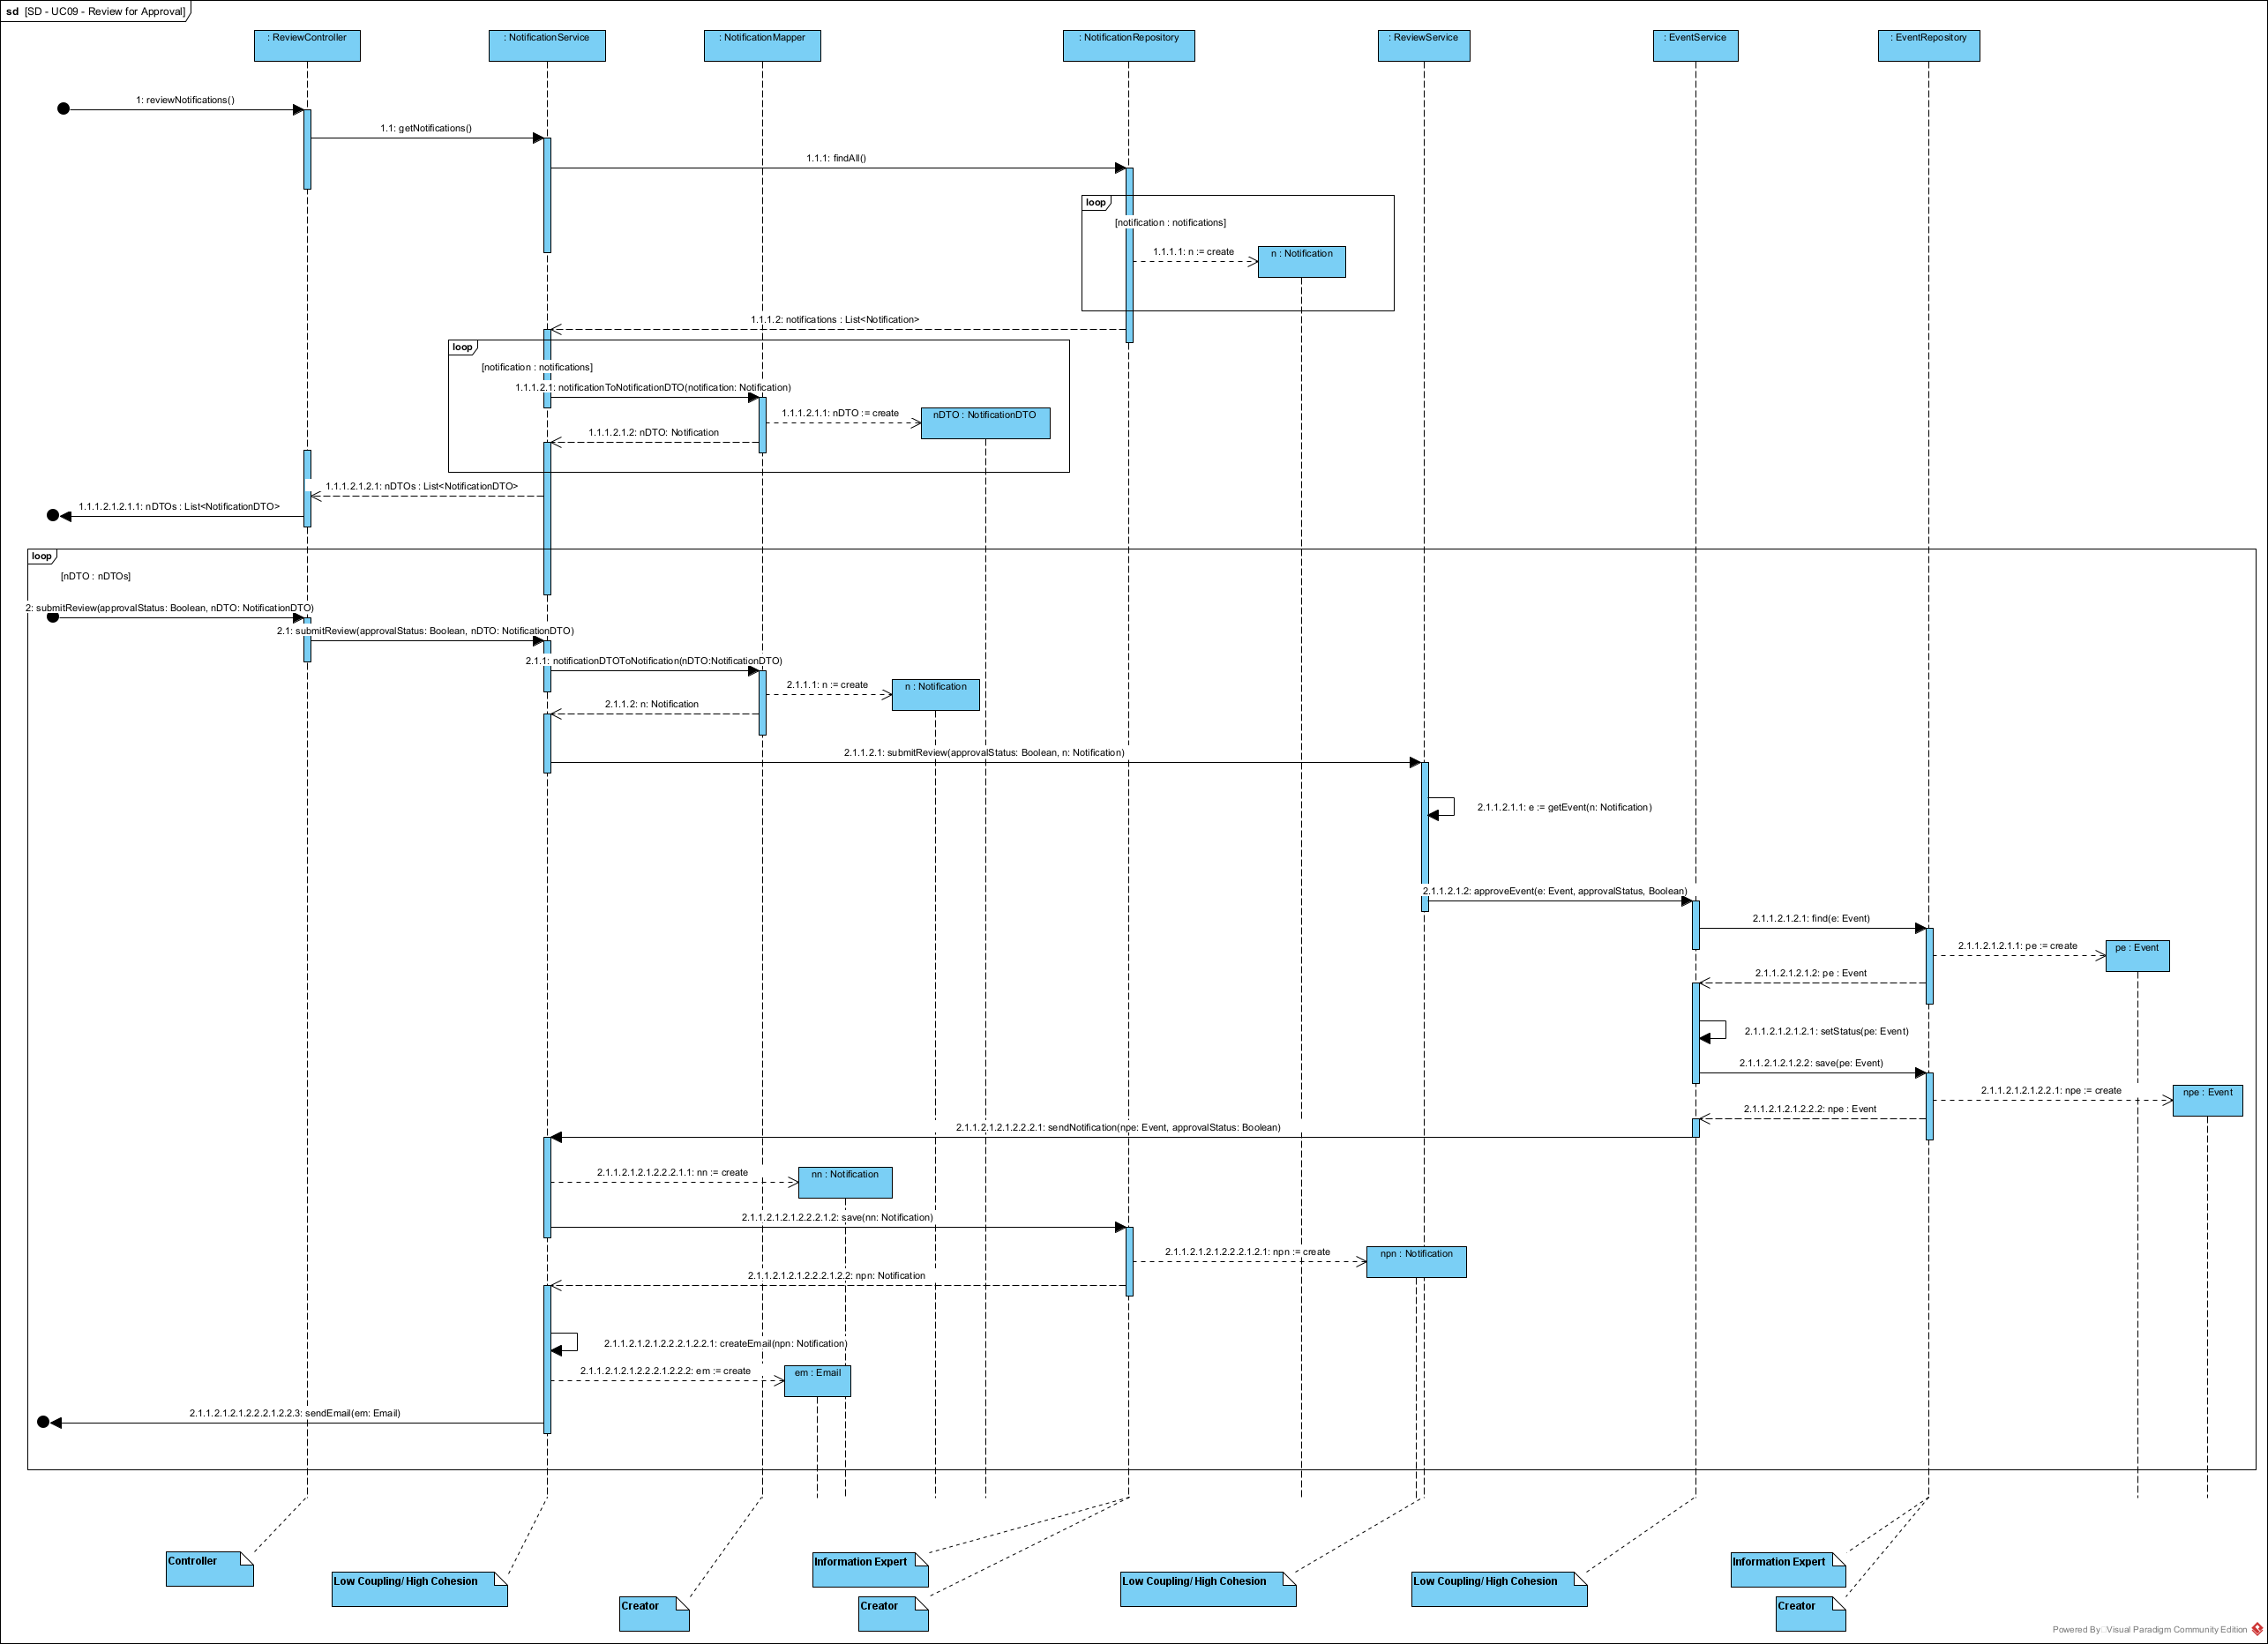
\includegraphics[scale=0.27]{images/SD-UC09-ReviewForApproval.png}
        \captionof{figure}{Sequence Diagram: Review for Approval}
        \label{fig:SD-ReviewForApproval}
\subsubsection{Sequence Diagram: Edit Post}
        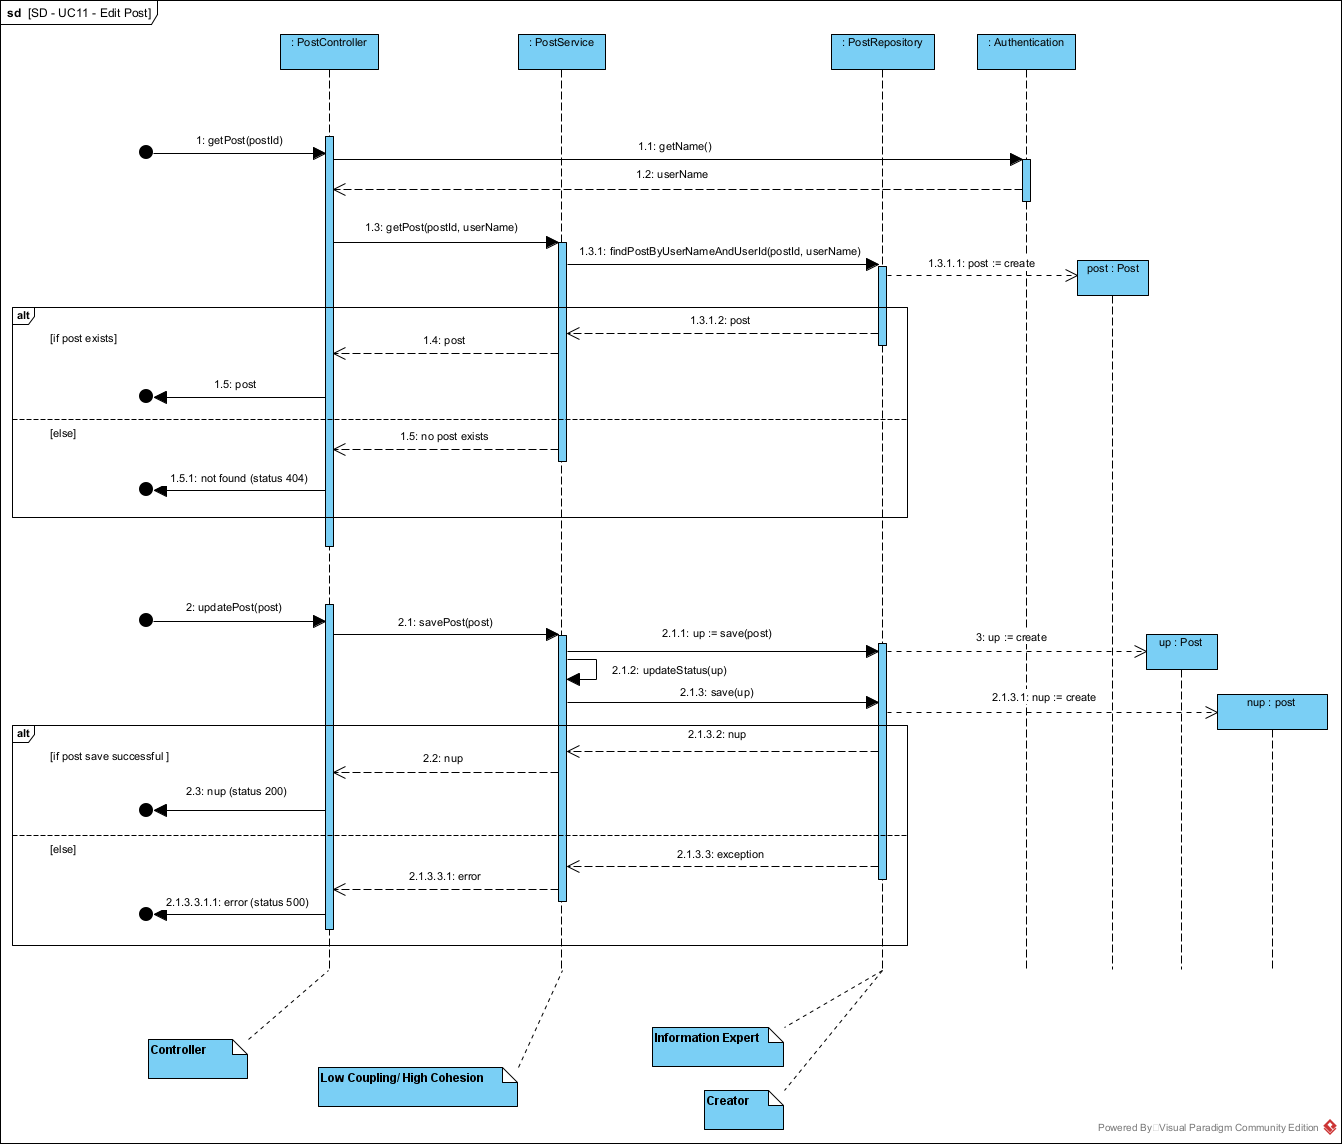
\includegraphics[scale=0.5]{images/SD-UC11-EditPost.png}
        \captionof{figure}{Sequence Diagram: Edit Post}
        \label{fig:SD-EditPost}
\subsubsection{Sequence Diagram: Manage Displayed Media}
        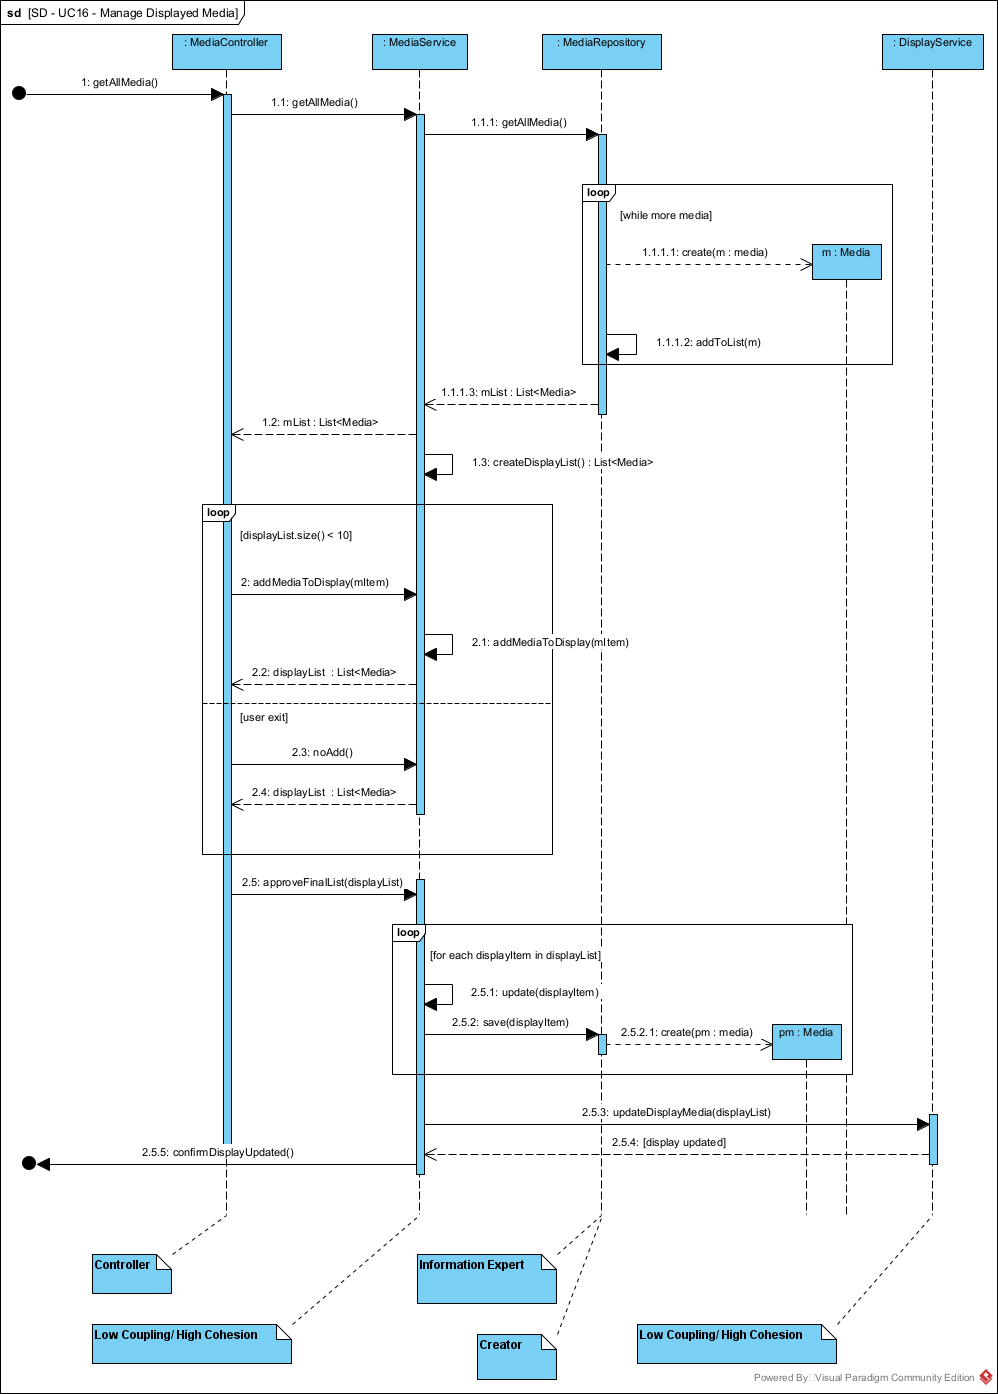
\includegraphics[scale=0.55]{images/SD-UC16-ManageDisplayedMedia.png}
        \captionof{figure}{Sequence Diagram: Manage Displayed Media}
        \label{fig:SD-ManageDisplayedMedia}
\subsubsection{Sequence Diagram: Add Page to Event}
        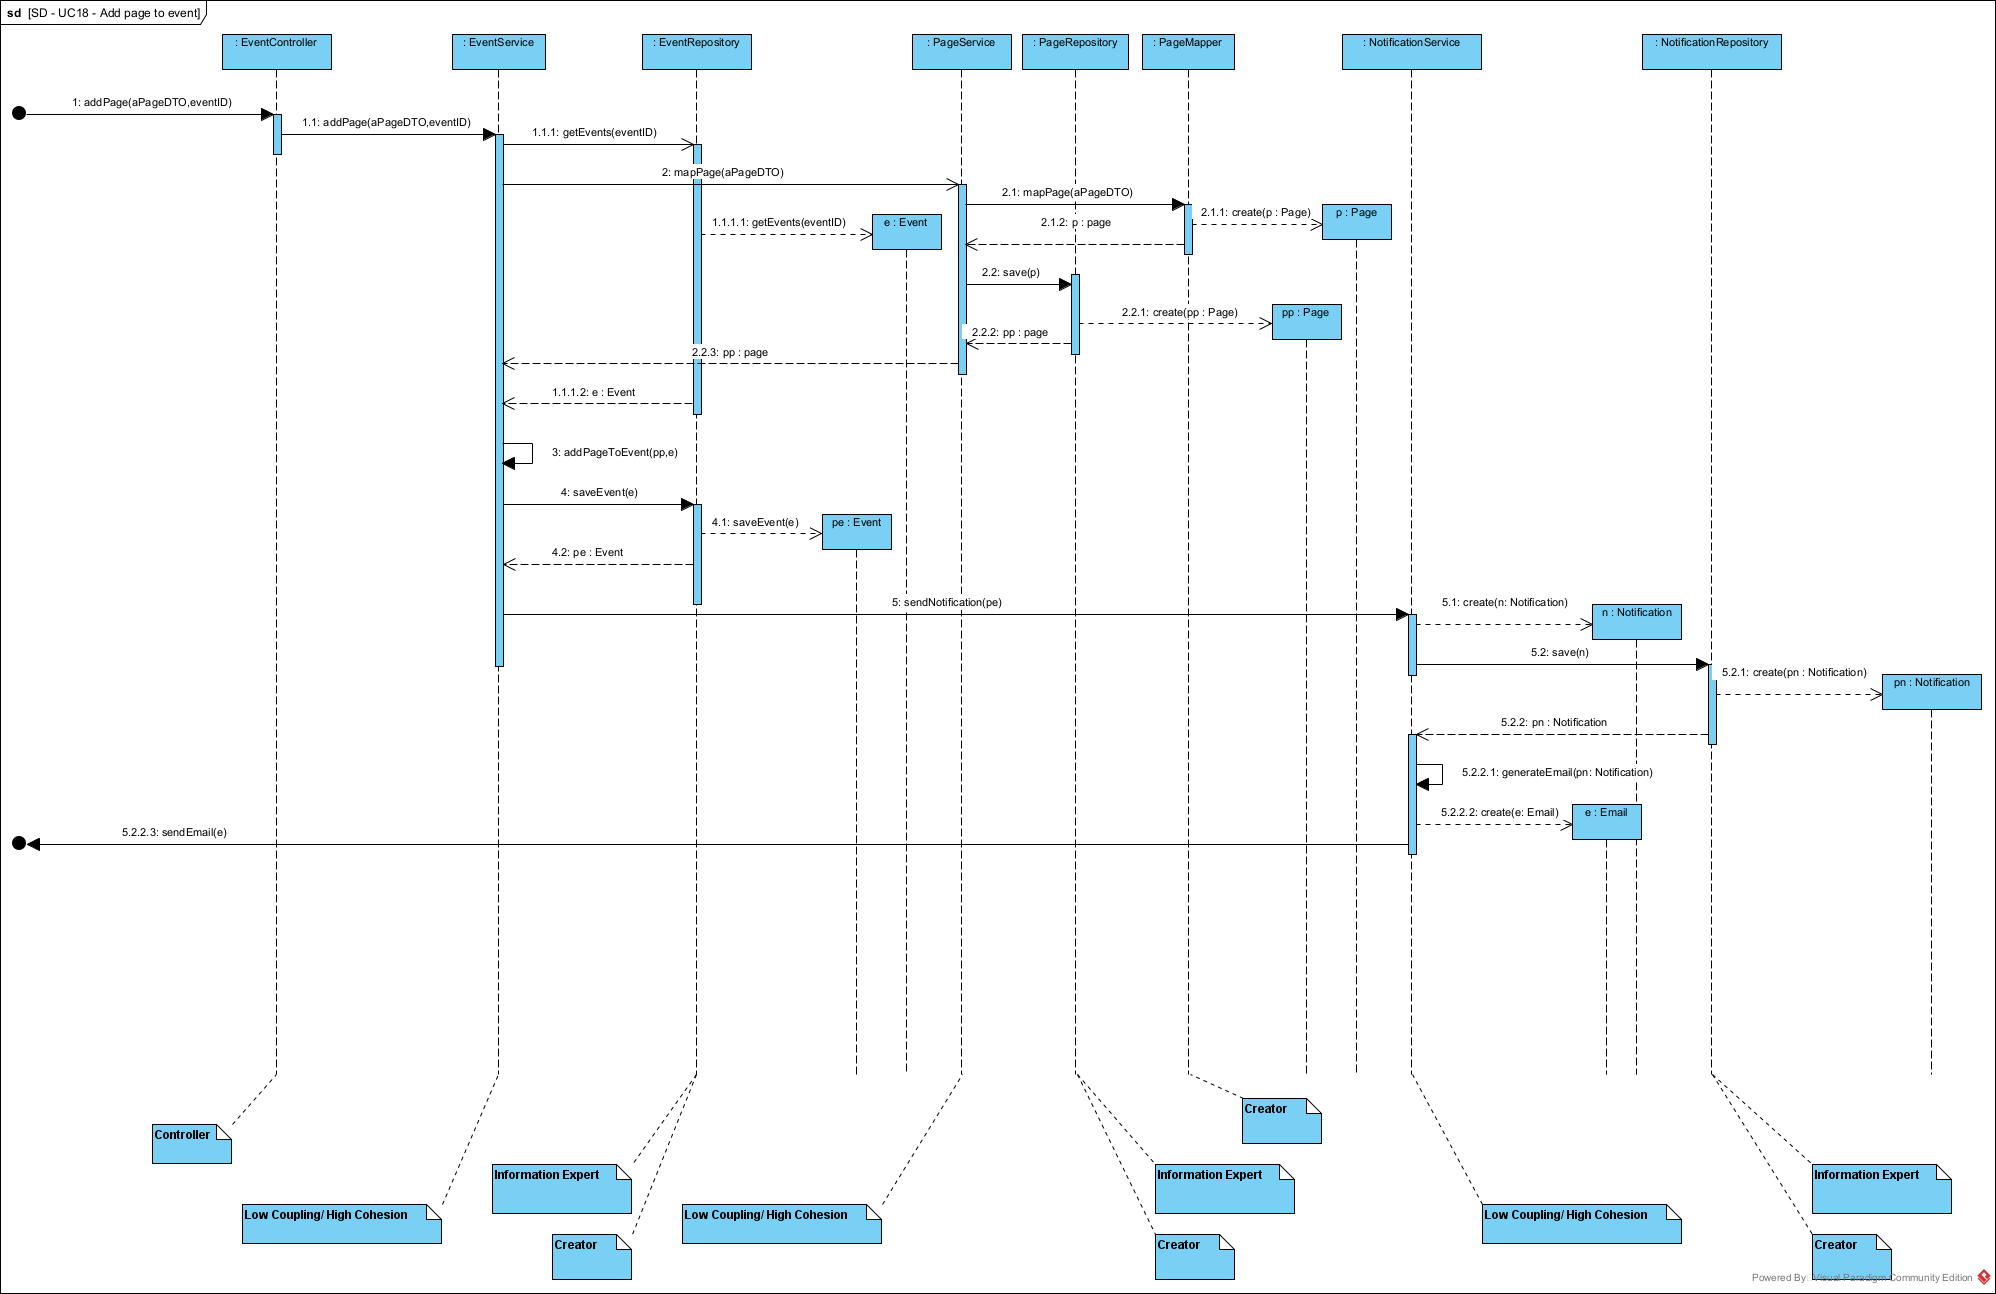
\includegraphics[scale=0.35]{images/SD-UC18-AddPageToEvent.png}
        \captionof{figure}{Sequence Diagram: Add page to Event}
        \label{fig:SD-AddPageToEvent}